%%%% fs-run-time-data-flow  FlameStream data flow

\label {fs-model}

The key concept of \FlameStream\ model is a datastream. It is a sequence of discrete events described by data items, internally represented as 
$(Payload, Meta).$
The $payload$ is processed by a  user-defined code, while $Meta$ is handled with \FlameStream\ engine. In particular
the primary purpose of the meta-information is to impose the total order on data items. 
The  $Meta$ is assigned at the entry (called {\em  front}) and is discared at the {\em barrier} just before the exit. 

% \subsection{Computational flow}
The stream processing is specified by a logical execution graph. 
Each node of the graph represents a single operation on data items, and edges describe the routing of data items between operations.  
Our model allows cycles in the graph while such graphs are commonly assumed to be acyclic (DAGs) 
~\cite{Zaharia:2016:ASU:3013530.2934664, Carbone:2017:SMA:3137765.3137777}. 
The cycles are required for specification of certain computations (e.g MapReduce-based) with our spartan set of operation types (outlined below).
%Moreover, as we show further, there are cases when cycles are required, e.g., for MapReduce-based algorithms. 
Figure~\ref{logical-graph-figure} shows the example of logical execution graph.

% \subsection{Physical deployment and partitioning}
A distributed hardware environment is modelled as a set of {\em worker} processes. 
Each the workers executes logical execution graph and has an assigned range of hash values used for physical routing of data items to workers. 
%An integer interval (hash range) is assigned to every worker. Intervals are not intersected and cover the range of 32-bit signed integer.
%
Each operation input has a user-provided hash function called {\it balancing function}. This function is applied to the payload of data items and determines partitioning before each operation. After that, the data items are sent to the worker, which is responsible for the associated hash range. Therefore, load balancing explicitly depends on the user-defined balancing functions. 
%This allows the developer to determine optimal balancing which requires the knowledge of the payload distribution. The system optimizes the hash ranges assignment according to the processing statistics. 

\begin{figure}[ht]
  \centering
  \begin{minipage}[b]{.5\textwidth}
    \centering
    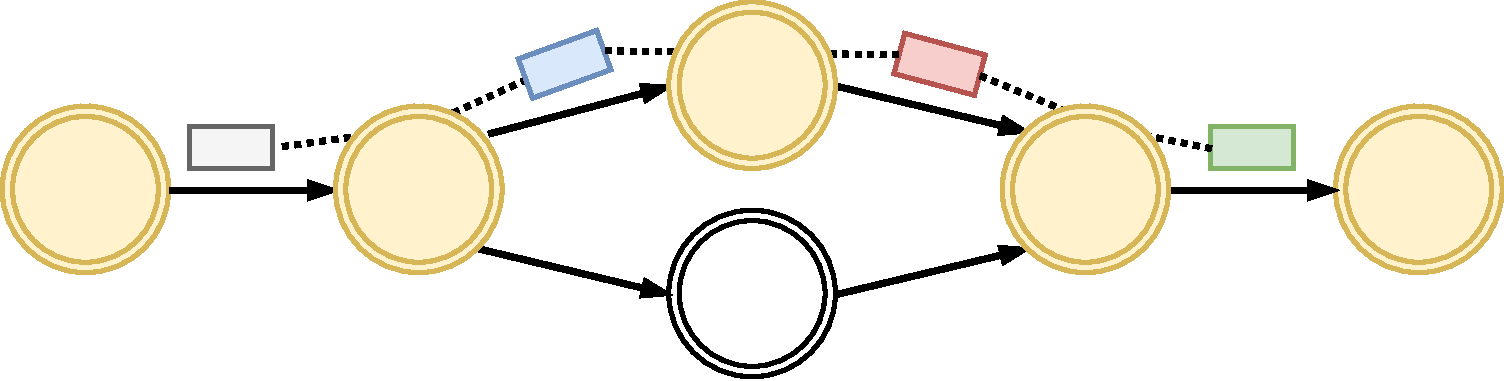
\includegraphics[width=\linewidth]{pics/logical-graph}
    \caption{A logical execution  graph}
    \label{logical-graph-figure}
  \end{minipage}%
  \begin{minipage}[b]{.5\textwidth}
    \centering
    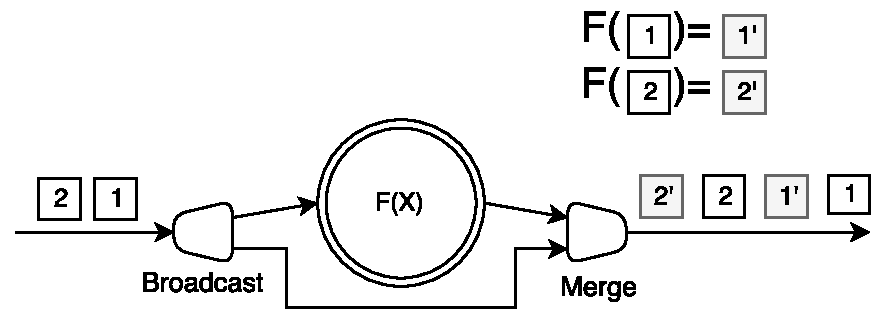
\includegraphics[width=\linewidth]{pics/ordering}
    \caption{The ordering model}
    \label{ordering}
  \end{minipage}
\end{figure}

\subsection{Ordering model}

We assume that there is a total order on data items. 
Ordering is preserved when an item is going through the operations. 
More precisely, the order of output items is the same as the order of corresponding input items. 
If more than one item is generated, they are inserted in output stream sequentially. 
Moreover, the output follows corresponding input but precedes the next item. 
Without diving into details, it should be noted that the order of items is maintained across different fronts.

The ordering is illustrated  in Figure~\ref{ordering}. Data item with payload $1'$ is the derivative of the item with payload $1$, according to operation $F$. The same is for items with payloads $2'$ and $2$. After merge operation, the order between $1$ and $2$ is preserved. Furthermore, $1'$ follows $1$, and $2'$ follows $2$.  

%  We assume that input items of the operations are strictly ordered.

\subsection{Operations}

The list of available operations includes:

{\bf Map} applies a user-defined function to the payload of an input item. This function returns a sequence of data items with transformed payloads. An output sequence can be empty.

{\bf Broadcast} replicates an input item to the specified number of operations.

{\bf Merge} operation is initialized with the specified number of input nodes. It sends all incoming data to the output.

{\bf Grouping} has a {\it window size} parameter. Grouping stores input items into distinct buckets by the value of the input balancing function applied to the payload. When the next item arrives at the grouping, it is appended to the corresponding bucket. Each time the grouping outputs window-sized {\it tuple item}, which consists of the most recent (in terms of the meta-information) items of this bucket. If the size of the bucket is less than the window, all items of the bucket are taken. Grouping is the only operation that has a state.

The following example illustrates the semantics of the operation. The grouping accepts items with payload represented as natural numbers: 1,2,3, etc. The hash function returns 1 if the number is even and 0 otherwise. If the window is set to 3, the output is:

\[(1), (2), (1|3), (2|4), (1|3|5), (2|4|6), (3|5|7), (4|6|8)...\]

There are two important properties of the grouping operation: the output tuple is identified by its last element, the results among items with different values of a hash function are independent.

\subsection{User-defined parameters}

A user can set up the following parameters:

\begin{enumerate}
  \item{Computational flow}
  \item{Balancing functions of the inputs}
  \item{Map functions}
  \item{Grouping windows}
\end{enumerate}

These parameters can produce more than one graph, which can yield equivalent results. Choosing among them is a performance optimization problem that relies on the system.
It is important to mention that there are no parameters for state-management. Therefore, business-logic is stateless. Nevertheless, the operations set is enough to implement any MapReduce transformation as shown in the next section.
